% Name: Process memory layout
% Description: The segments of a process's address space, with the heap growing up and the stack growing down.
% Tags: memory layout, heap, stack, operating systems

\usetikzlibrary{arrows.meta}

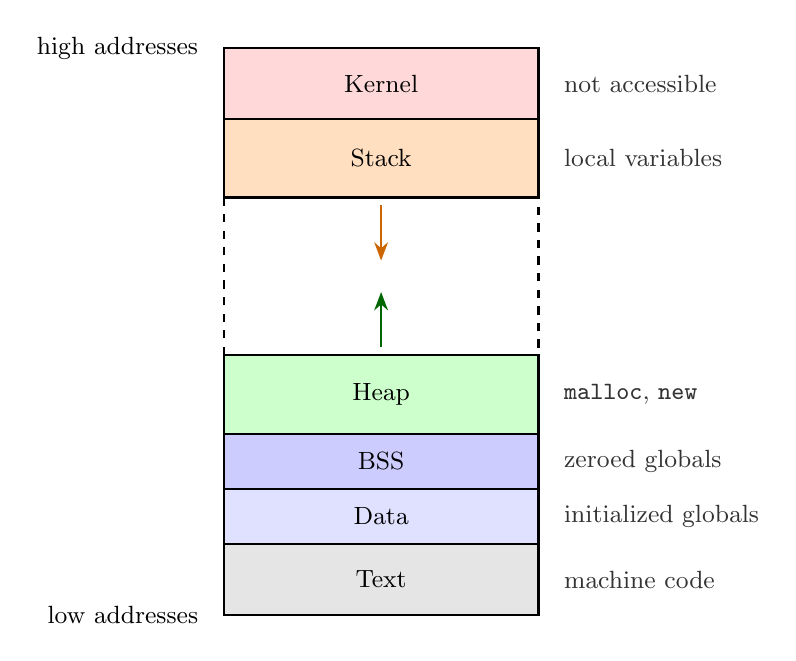
\begin{tikzpicture}[every node/.style={font=\small}, >={Stealth}]
  \foreach \lo/\hi/\c/\name/\note in {
    0/0.9/gray!20/Text/machine code,
    0.9/1.6/blue!12/Data/initialized globals,
    1.6/2.3/blue!20/BSS/zeroed globals,
    2.3/3.3/green!20/Heap/{\texttt{malloc}, \texttt{new}},
    5.3/6.3/orange!25/Stack/local variables,
    6.3/7.2/red!15/Kernel/not accessible%
  } {
    \draw[thick, fill=\c] (0,\lo) rectangle (4,\hi);
    \node at (2,{(\lo+\hi)/2}) {\name};
    \node[right, gray!40!black] at (4.2,{(\lo+\hi)/2}) {\note};
  }
  \draw[thick, dashed] (0,3.3) rectangle (4,5.3);
  \draw[->, thick, green!40!black] (2,3.4) -- (2,4.1);
  \draw[->, thick, orange!80!black] (2,5.2) -- (2,4.5);
  \node[left] at (-0.2,0) {low addresses};
  \node[left] at (-0.2,7.2) {high addresses};
\end{tikzpicture}
